\section{Telemetry data module}

\subsection{Client Service}
  Receives data from the telemetry server middleware module.

\subsection{Data Processing Functions}
  Receives data from client service and splits it into relevant, useful categories
  such as gyroscopic data, acceleration, etc.

  Performs functions on data as necessary to make it useful for outside modules
  such as the EFV module.

\subsection{Error Checking}
  Performs functions on data as necessary to indicate strength and integrity
  of data and signals.

\subsection{Display}
  Displays pertinent telemetry data to relevant views, in respective
  HTML ids and tags.

  Displays graphical representations of numeric data in real time.
  Organizes information in an easy to read format.

  Responsible for ``at-a-glance'' view.

\begin{figure}[h!]
\centering
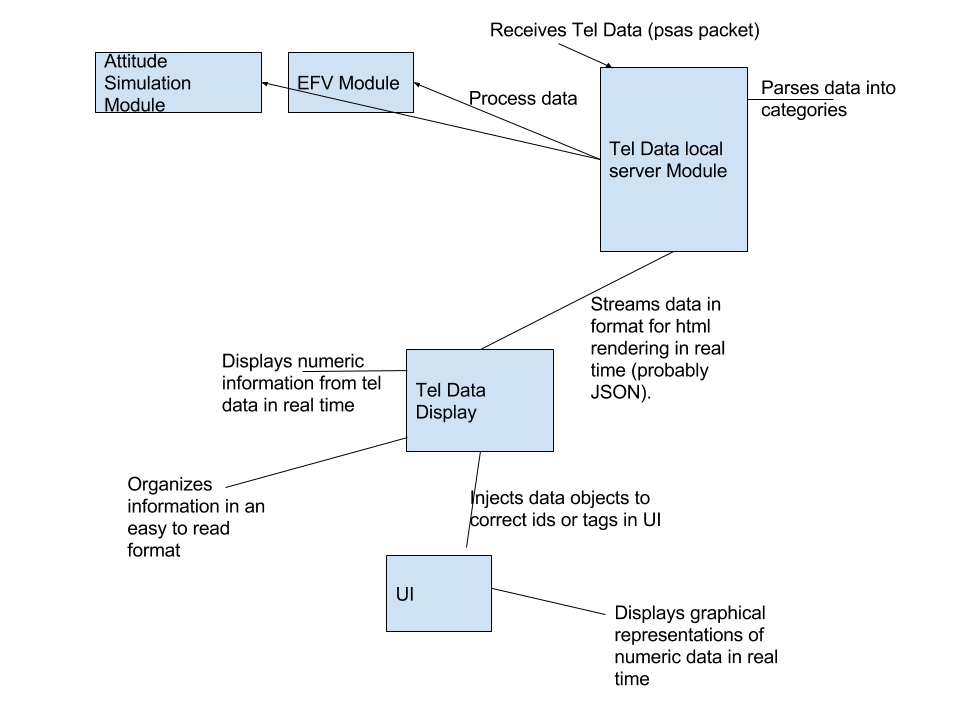
\includegraphics[scale=.45]{imgs/tel-data-module.png}
\caption{Telemetry Module Architecture Plan \label{tel}}
\end{figure}
